\documentclass[a4paper,USenglish]{article}
 
 \usepackage{microtype}%if unwanted, comment out or use option "draft"
 
 \usepackage{authblk}
 
 %\pdfpagesattr{/CropBox [80 80 523 780]}
 \pdfoutput=1
 \usepackage[utf8]{inputenc}
 %\usepackage{microtype}
 \usepackage{amsmath}
 \usepackage{amsthm}
 \usepackage{amssymb}
 \usepackage{float}
 \usepackage[algoruled,linesnumbered,noend]{algorithm2e}
 \usepackage{relsize}
 \usepackage{enumitem}
 \usepackage{cite}
 \usepackage{multirow}
 \usepackage{caption}
 %\usepackage{subcaption}
 \usepackage{url}
 \usepackage{xspace}
 \usepackage{graphicx}
 \usepackage{booktabs}
 \usepackage{mathcomp}
 \usepackage{ifdraft}
 \usepackage{standalone}
 \usepackage[external]{forest}
 
 % REMOVE BEFORE SUBMISSION - begin part
 \usepackage{verbatim}
 \newcommand{\notaestesa}[2]{%
   \marginpar{\color{red!75!black}\textbf{\texttimes}}%
   {\color{red!75!black}%
     [\,\textbullet\,\textsf{\textbf{#1:}} %
     \textsf{\footnotesize#2}\,\textbullet\,]}%
 }
 \newcommand{\mynote}[2]{%
   \marginpar{\color{red!75!black}\textbf{\texttimes}}%
   {\color{red!75!black}%
     [\,\textbullet\,\textsf{\textbf{#1:}} %
     \textsf{\footnotesize#2}\,\textbullet\,]}%
 }
 
 \usepackage{tikz}
 \usetikzlibrary{shapes,arrows}
 %\usetikzlibrary{snakes}
 \usetikzlibrary{positioning,patterns}
 \usepackage{ifpdf}\usepackage{datetime}
 \ifpdf%
 \pdfinfo{%
   /Author (Author1;Author2)
   /Title (Title)
   /Keywords (perfect phylogeny;persistent perfect phylogeny)
   /CreationDate (D:\pdfdate)
 }
 \fi
 
 
\newcommand{\grb}{\ensuremath{G_{RB}}\xspace}
\newcommand{\ie}{i.e.,~}
\newcommand{\eg}{e.g.,~}
\newcommand{\wrt}{w.r.t.~}
\newcommand{\IH}[1]{\textbf{\color{red}{[IH:#1]}}}
 
 
 
\newtheorem{theorem}{Theorem}
\newtheorem{lemma}[theorem]{Lemma}
\newtheorem{proposition}[theorem]{Proposition}
\newtheorem{Observation}[theorem]{Observation}
\newtheorem{corollary}[theorem]{Corollary}
\newtheorem{Claim}[theorem]{Claim}
\newtheorem{property}[theorem]{Property}
\theoremstyle{definition}
\newtheorem{definition}{Definition}
\newtheorem{Problem}{Problem}
\newtheorem{Example}{Example}[section]


\begin{document}

\title{Inferring Cancer Progression from Single-cell via ILP}
% \author[Ciccolella \textit{et~al}]{Simone Ciccolella\,$^{1,}$\footnote{to whom correspondence should be addressed}, Mauricio Soto Gomez\,$^{1}$, Murray Patterson\,$^{1}$, Gianluca Della Vedova\,$^{1}$, Iman Hajirasouliha\,$^{2,3}$ and Paola Bonizzoni\,$^{1}$}
% \address{$^{1}$Department of Computer Science, Systems and Communication, Univ. Milano-Bicocca, Milan, Italy\\
% $^{2}$Institute for Computational Biomedicine, Department of Physiology and Biophysics, Weill Cornell Medicine of Cornell University, NY, USA\\
% $^{3}$Englander Institute for Precision Medicine, The Meyer Cancer Center, Weill Cornell Medicine, NY, US}

\maketitle

\begin{abstract}
\textbf{Motivation:} In recent years, the well-known Infinite Sites Assumption (ISA) has been a fundamental feature of computational methods devised for reconstructing tumor phylogenies and inferring cancer progression. However, recent studies leveraging Single Cell Sequencing (SCS) techniques have shown evidence of widespread recurrence and loss of mutations in several tumor samples, an observation which essentially violates a strict ISA (\eg,~\cite{Kuipers13102017}).\\
\textbf{Results:} We present the \texttt{SASC} (Simulated Annealing Single Cell inference) tool, a new model and robust framework based on simulated annealing for the inference of cancer progression from SCS data.
	Our main objective is to overcome the limitations of the Infinite Sites Assumption by introducing a version of the Dollo parsimony model which indeed allows the deletion of mutations from the evolutionary history of the tumor. 
	We demonstrate that \texttt{SASC} achieves high levels of accuracy when tested on both simulated and real data sets and in comparison with other available methods.\\
\textbf{Availability:} The General Parsimony Phylogeny from Single-cell (\texttt{gpps})
tool is open source and available at   \url{https://github.com/AlgoLab/gppf}.\\
% \textbf{Contact:} \href{s.ciccolella@campus.unimib.it}{s.ciccolella@campus.unimib.it}
%\textbf{Supplementary information:} Supplementary data are available at \textit{Bioinformatics}online.}
\end{abstract}

\section{Introduction}

Recent developments of targeted therapies for cancer patients rely on the accurate inference of the clonal evolution and progression of the particular cancer. As discussed in several recent studies such as~\cite{Morrissy2016} and~\cite{Wang2016}, understanding the order of accumulation and prevalence of somatic mutations during cancer progression can help better devise therapeutic strategies.

Most of the available techniques for inferring cancer progression rely on data from next-generation bulk sequencing experiments, where only a proportion of observable mutations from a large amount of cells is obtained, without the distinction of the cells that carry them. In recent years, many computational approaches have been developed for the analysis of bulk-sequencing data with the purpose of inferring tumoral subclonal decomposition and reconstructing tumor phylogenies (trees)~\cite{Strino2013,Jiao2014,Hajirasouliha2014,Yuan2015,Popic2015,citup,El-Kebir2016,marass2016,doi:10.1093/bioinformatics/btx270,Bonizzoni:2017:BPP:3107411.3107441}.

Single Cell Sequencing (SCS) promises to deliver the best resolution for understanding the underlying causes of cancer progression. However, it is still difficult and expensive to perform SCS experiments with a high degree of confidence or robustness. The techniques available nowadays are producing datasets which contain a high amount of noise that include allelic dropout (false negatives) and missing values, due to lack of read coverage and false positive calls -- even in a relatively small fraction. Although this sequencing technology is rapidly improving, and some issues such as the presence of doublets are slowly fading away, it is important to develop methods that are able to infer cancer progression despite the lack of accuracy in the data produced by current SCS techniques.

Various methods have been developed for this purpose~\cite{Jahn2016,Ross2016, Zafar2017}, some of them introducing a hybrid approach of combining both SCS and VAF data~\cite{Ramazzotti132183, Malikic234914, Salehi2017}.  Most of these methods, however, rely on the Infinite Sites Assumption (ISA), which states that a mutation is acquired at most once in the phylogeny and is never lost. The ISA was introduced in~\cite{Kimura1969} by Kimura in 1969: one of the pioneering papers of the neutral model of the evolution of species. This simplifying assumption also leads to a computationally tractable model of evolution~\cite{gusfield1991} -- something that is safe to make in this setting. Cancer progression, however, is a very fast and aggressive form of evolution with limited data supporting neutral evolution~\cite{DAVIS2017151}, with some studies showing rather the evidence of selection~\cite{Bignell2010,DAVIS2017151} -- something that is particularly true in tumour samples after a relapse~\cite{Ding2012,Gillies2012,DAVIS2017151}, where the tumour has already been highly selected by the therapy targeted to destroy it.
%\
Thus, one would be expect that we must abandon the strict Infinite Sites Assumption in this setting, and indeed this is the case, as more and more recent studies are demonstrating that the ISA does not always hold~\cite{Kuipers13102017,Brown2017,Bignell2010}. In~\cite{Brown2017}, the authors find that large deletions on several branches of a tree can span a shared locus, and
thus a given mutation may be deleted independently multiple times.  In~\cite{Bignell2010}, the authors show that in certain cases, homozygous deletions in cancer genomes can even provide a selective growth advantage. Each (independent) deletion of an acquired mutation takes us further away from the ISA. Some recent methods such as TRaIT~\cite{Ramazzotti132183} and SiFit~\cite{Zafar2017}  permit violations of the ISA, in particular they allow deletions of mutations without specifying a particular model of evolution.  While this is a start, there is a need to develop more general methods, based relaxing the ISA -- something that is not robust to even a single back-mutation.

The Dollo model~\cite{Rogozin2006} is designed exactly for cases where stricter models like the one based on the ISA may not provide a solution.  In particular, while it still constrains that a mutation can only be \textit{acquired} once, it allows any number of independent losses of the mutation -- a model that is very pertinent in light of the above cases~\cite{Kuipers13102017,Brown2017,Bignell2010} for the ISA not holding. Of course, the Dollo model does not have the convenient computational tractability of the perfect phylogeny model~\cite{gusfield1991}. However, if we restrict the number of losses of any mutation to 1 or 2 (rather than strictly 0), the resulting solution space is still small enough to search in a practical amount of time.

Here we propose the Simulated Annealing Single Cell inference (\texttt{SASC}) tool, a maximum likelihood tree search framework that allows violations of the ISA, in the form of deletions of mutations, by incorporating the Dollo parsimony model~\cite{Farris_1977}.

\section{Formulation of the tree reconstruction problem}
As mentioned before, cancer progression reconstruction can be modeled as a
character-based phylogeny reconstruction problem in which mutations
are represented by the presence/absence of characters in different 
cell groups represented by the species.
\begin{figure}[tb]
  \begin{minipage}{0.4\linewidth}
     \includegraphics[scale=.4]{img/dollo_example}
\end{minipage}
\begin{minipage}{0.3\linewidth}
        \begin{tabular}[!t]{c|ccccccc}
             & a & b & c & d & e & f & g  \\ \hline
            $s_1$ & 1 & 1 & 1 & 0 & 0 & 0 & 0 \\
            $s_2$ & 1 & 0 & 0 & 0 & 1 & 0 & 0 \\
            $s_3$ & 0 & 1 & 0 & 1 & 0 & 1 & 0 \\
            $s_4$ & 1 & 0 & 0 & 0 & 0 & 0 & 1
        \end{tabular}
        \end{minipage}
  \caption{Example of a binary matrix that does not allow a perfect phylogeny, since columns $a$ and $b$ are in conflict, i.e. the four gametes rule~\cite{gusfield1991}
  does not hold. The tree represents one of the possible Dollo phylogenies that explain the matrix.}
\label{fig:dollo}
\end{figure}

The input is an $n \times m$ ternary matrix $I_{ij}$, where entry $I_{ij}=0$ indicates
that the sequence of cell $i$ does not have mutation $j$, $I_{ij}=1$ indicates the presence of mutation $j$ in the sequence of cell $i$, and a 2 indicates
that there is not enough information on the presence/absence of mutation $j$ in cell $i$.
Uncertainty about the presence of a mutation in a cell is a consequence of insufficient coverage in the sequencing. 

However, uncertainty is not the only issue in the sequencing process:
the input matrix $I$ also contains false positives and false negatives. 
We assume that these error occur independently and uniformly across 
all the (known) entries of $I$. 
Namely, if $E_{ij}$ denotes the estimated $n\times m$ output matrix, \ie the binary matrix without errors and noise estimated by the algorithm,
$\alpha$ denotes the false negative rate and $\beta$ denotes the false positive rate; then for each $ij$ entry of $E$ the following holds:
\begin{itemize}
    \item $P(I_{ij} = 0|E_{ij} = 0) = 1- \beta$
    \item $P(I_{ij} = 1|E_{ij} = 0) = \beta$
    \item $P(I_{ij} = 1|E_{ij} = 1) = 1- \alpha$
    \item $P(I_{ij} = 0|E_{ij} = 1) = \alpha$
\end{itemize}

We aim to find a matrix $E$ that maximizes the following function 
$$
    \mbox{max } P(I|E) = \prod_{i}^{n} \prod_{j}^{m} P(I_{ij}|E_{ij}).
$$
In other words, we attempt to maximize the likelihood of the observed matrix $I$~\cite{Jahn2016}.
We point out that the values of the unknown entries of the input matrix 
do not affect in the objective function.
Thus, $P(I_{ij} = 2|E_{ij} = 1) = P(I_{ij} = 2|E_{ij} = 0) = 1$.

Moreover, since we are interested in the reconstruction of the evolutionary history 
of the input cells, we must provide, together with
matrix $E$, a phylogenetic tree which explains the evolution 
of the mutations present in the cells of the output matrix.

A phylogenetic tree is defined as a rooted labeled tree $T$ in 
which the label set corresponds to a set of characters, and the 
leaves of $T$ have the void label.
The state of a node is defined as the set of 
labels (characters) in the path from the root.
The state of each leaf $l$ of $T$ is naturally
represented by an $m$-dimensional binary vector, that
we denote $D(T,l)$, such that $D(T,l)_j=1$ if and
only if the $l$ contains the mutation $j$ and zero otherwise.

We say that the tree $T$ encodes a matrix $E$ 
if there exists a mapping $\sigma$ of the rows (cells) of $E$
as leaves of $T$ such that for every row $E_{i}=D(T,\sigma_i)$,
where $\sigma_i$ denotes the image of row $i$ by $\sigma$, 
\ie $\sigma_i$ is the node in the phylogenetic tree to which cell $i$ is attached as leaf.
\begin{figure}[!tb]
  \begin{minipage}{0.7\linewidth}
    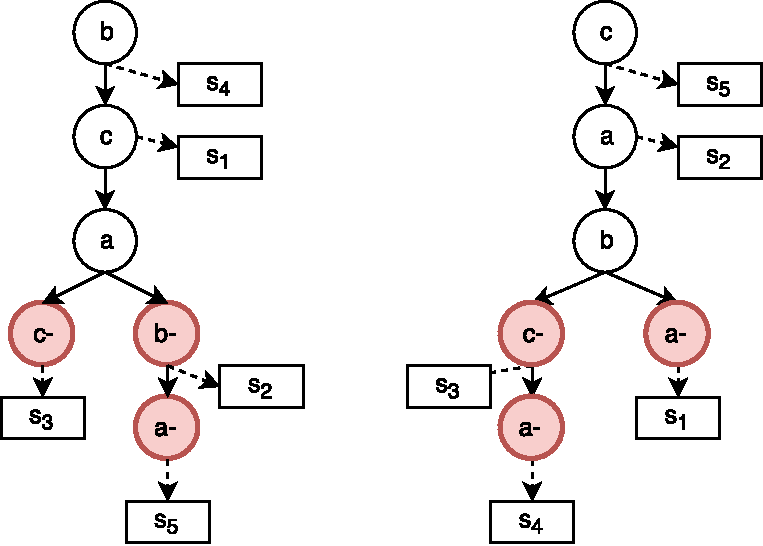
\includegraphics[scale=.4]{img/dollo_non_unique}
\end{minipage}
\begin{minipage}{0.2\linewidth}
    \begin{tabular}[!t]{c|ccc}
            & a & b & c \\ \hline
            $s_1$ & 0 & 1 & 1 \\
            $s_2$ & 1 & 0 & 1 \\
            $s_3$ & 1 & 1 & 0 \\
            $s_4$ & 0 & 1 & 0 \\
            $s_5$ & 0 & 0 & 1
\end{tabular}
\end{minipage}
\caption{Example of two Dollo phylogenies that explain the same binary matrix. 
It is important to notice that the ancestral order of mutations $c,a$ and $b$ is inverted but the two different trees can equally explain the input binary matrix. In fact, in a Dollo phylogeny the order of two mutations can be inverted and, thank to the introduction of deletions, they could both be correct solutions for a given input.
}
\label{fig:dollo_non_unique}
\end{figure}

We can express the likelihood of the matrix $E$ as: $P(I|E) = \prod_{i}^{n} \prod_{j}^{m} P(I_{ij} | D(T, \sigma_i)_j)$.
Since the involved probabilities are in [0,1] it is convenient to move to a (linear) log-likelihood maximization objective function of the form:
\begin{equation}
\label{eq:log-likelihood}
    \mbox{max } \sum_i^n \sum_j^m \log(P( I_{ij}| D(T, \sigma_i)_j))
\end{equation}

\subsection{Introduction of Dollo($k$) model}
\label{sec:intro_dollok}
The Dollo parsimony rule can be interpreted as the impossibility of 
having an identical mutation in the
evolutionary trajectory.
This rule can be translated in the phylogeny tree model as the unique introduction of 
any single mutation but any number of deletions of this mutation. 

From an algorithmic point of view,
the phylogeny reconstruction model 
with a Dollo evolutionary model is 
an NP-complete problem~\cite{BKW95,DAY198633}.
A hierarchical chain of restricted versions of the model can be obtained by bounding the number of deletions for each character.
We denote as Dollo($k$) the evolutionary model in which each mutation can be acquired exactly once and can be lost at most $k$ times. 
In this way Dollo(0) and Dollo(1) correspond to the perfect and persistent phylogeny models, respectively.
In the tree generation process for the Dollo($k$) model ($k>0)$ we are required to augment the phylogenic tree $T$ representing the cancer progression by adding nodes which represent the loss of a mutation, i.e. a node labelled $p^-_l$, representing the $l$-th loss of mutation $p$. 
As a consequence, the function $D(T, \sigma)$ needs to be slightly modified to take account of the losses. The genotype profile of a row $i$ is then given by the mutations acquired in the path from the root to the parent of $\sigma_i$ minus all of the potential losses encountered in the path.
We stress the fact that, when deletions are introduced, 
the set of feasible phylogenies which represent a given solution is no longer unique as in the case of Perfect phylogeny. We can see that switching the labels of nodes $b^-$ and $d^-$ in Figure~\ref{fig:dollo} produces a different tree which is still a solution of the proposed input matrix. 
Moreover we see that ancestral relationship between characters is different in both representations.
When the number of cells, mutations and possible deletions increases, and with the noise caused by false calls and missing entries, this problem is greatly amplified, causing the number of different cancer progression phylogenies which equally explain the same input, to explode. A more complex example can be seen in Figure~\ref{fig:dollo_non_unique} where a different order of mutations and a different set of deletions can equally explain a given input.

\section{Preliminaries}
\label{sec:preliminaries}



\subsection{The Incomplete Directed Perfect Phylogeny Problem}
\label{sec:idpp}

The character-based phylogeny reconstruction problems we study in this
  paper are constrained versions of the general Incomplete Directed
  Perfect  Phylogeny (IDP)~\cite{Peer_2004}.
The IDP problem asks for completing missing data in a binary matrix, where
  missing data are represented by the symbol $?$, in such a way that the
  completed matrix is explained by a perfect phylogeny.
More precisely, the input data is an $n\times m$ matrix $M_{?}$, where
  $M_{?}(i,j)\in \{0,1,?\}$ represents the absence, presence or
  uncertainty of a character $j$ in the species $i$ respectively.
If a solution  exists, then it consists of changing  each $?$ into $0$
  or $1$  obtaining a new  binary matrix  $M_{s}$ that has  a directed
  perfect phylogeny. 
 
A well  known characterization  of perfect  phylogenies states  that a
  binary matrix $M_{s}$ has a directed perfect phylogeny if and only if
  it has  no \emph{conflicting}  pair of columns ---  two columns  are in
  conflict  if  they contain  all  three configurations  $(0,1)$,
  $(1,0), (1,1)$ --- inducing the so-called forbidden matrix.
The problem of  determining if a binary  matrix has a perfect  phylogeny, and to
  compute  such  perfect  phylogeny  if possible,  has  a  linear-time
  algorithm~\cite{Gusfield91,Gusfield}. 
Interestingly, the IDP  problem has an efficient solution  given by an
  $O(mn\log^{2}(m+n))$-time algorithm~\cite{Peer_2004} when the
  phylogeny is directed, that  is the root is known (and  is the all $0$s
  vector), otherwise,  the problem of  deciding whether there  exists an
  unrooted    solution   of    the    incomplete    input   matrix    is
  NP-complete~\cite{steel1992complexity}.
There exists an ILP formulation for variants  of the IDP problem, where the main
  question is to complete missing data in an input matrix on $\{0,1,?\}$ with the
  goal of minimizing the conflicting pairs \cite{Gusfield2007}. 
Since finding  a perfect phylogeny is  easy, the main difficulty  in solving the
  IDP problem consists of replacing each $?$ with a $0$ or a $1$ to minimize the
  number of conflicting pairs of columns.
%
\subsection{ILP formulation for the IDP}
\label{sec:ilp}
 In this section we revisit the ILP formulation proposed~\cite{Gusfield2007} for the IDP problem.
%
The input of the problem is an incomplete $n\times m$ matrix $M_?$.
The goal is to decide if there exists a completion of the unknown
entries  of $M_?$ resulting in
a (complete) matrix  admitting a Perfect Phylogeny.
The main  strategy of  this approach  is to state  the problem  as the
  minimization of the conflicts between pairs of characters. 
Thus, in virtue of the  Perfect Phylogeny Theorem, the IDP problem
will have a solution if and only if the cost of the minimization problem
is zero.  

% In what follows, we  briefly explain the key elements of the  ILP and we discuss
% the required changes for its use in the MIDPP problem.

\subsubsection{Variables}
  \label{sec:ILP_variables}  
A binary variable $Y(i,j)$ is defined for each unknown position of $M_?$.
With an abuse of notation, $Y(i,j)$ will be  a constant for every known
  position of the matrix of value  $M_?(i,j)$.  
Since the objective is to determine if two columns are in conflict,
  for every pair of columns $p,q$ we define a  binary variable $C(p,q)$
  which indicates the existence of a conflict between these two columns.
To establish if two columns are in conflict, we introduce the binary variables 
   $B(p,q,a,b)$, which  are defined for each pair of columns $(p,q)$ and for each
   possible  pair  of  values  $(a,b)\in \{0,1\}^2$.
The variable $B(p,q,a,b)$ indicates if for the (ordered) pair of columns $(p,q)$
  there  exists a row $i$ where $Y(i,p)=a$ and $Y(i,q)=b$.
Just as for the variable $Y(i,j)$, if there exists a row of the matrix such that 
  $Y(i,p)=a$ and $Y(j,q)=b$, then $B(p,q,a,b)=1$.

\subsubsection{Inequalities}
\label{sec:ILP_ineq}
For each pair $(p,q)$ of columns, for each pair $(a,b)\in
\{(1,0),(0,1),(1,1)\} $, and for each species $i$, the following set of inequalities 
\begin{equation}\label{eq:B}
   B(p,q,a,b)\ge 1-[a+(-1)^{a} Y(i,p)]-[b+(-1)^{b}
  Y(i,q)]
  \end{equation}
  force the variable $B(p,q,a,b)$ to be $1$ if and only if the columns $p,q$
  exhibit the pair $(a,b)$ in some row $i$.
 % We denote this set of constraints for an input matrix $M$ by $\mathcal B(M)$.  
  On the other hand, the following set of inequalities
  %, denoted by $\mathcal C(M)$, 
 forces  variables  $C(p,q)$ to  be  $1$  when characters  $p$  and  $q$ are  in
 conflict:  
\begin{equation}\label{eq:C} 
  C(p, q) \ge B(p,q,0,1) + B(p,q,1,0) + B(p,q,1,1)- 2  
\end{equation}

%\notaestesa{paola}{the following sentence is not clear to me...please specify}
% In  the  following sections  we  extend  this  formulation for  finding  minimal
% conflict completions when more general phylogenetic models are considered.
% Nevertheless, in the $\mathcal P$-VAFF problem we are 
% mainly interested about feasible solutions with no conflicts, that is
% when $C(p,q)=0$ for all pair of characters $p$ and $q$.
Since we are mainly interested in feasible solutions with no conflicts,
we  will  consider  the   following  alternative  form  of  the  previous
constraint: 
\begin{equation}\label{eq:C=0}
   B(p,q,0,1) + B(p,q,1,0) + B(p,q,1,1)\le 2.  
\end{equation}
% \notaestesa{GDV}{ Mauricio, the equation above allows to remove the variables $ C(p,q)$
%   and to pick any objective function.
% Do you agree with removing $C(p,q)$?}

% \notaestesa{MS}{In fatti  per questo la  modifichiamo così. Ho lasciato  (2) per
%   essere fedele al lavoro di Gusfield che si descrive in questa parte}

%
\subsubsection{Objective Function} Since we aim to minimize
the number of conflicts,  the objective function is defined as
$\min\sum_{(p,q)}C(p,q)$.

By the previous discussion it is possible to state the problem of
finding a  completion with the  minimal number  of conflicts by  considering the
solution of the following minimization problem~\cite{Gusfield2007}: 
$
\min\sum_{(p,q)}C(p,q)\;\text{ s.t.}\;\eqref{eq:B}, \eqref{eq:C}.
$
We stress that that decision problem of determining if an incomplete matrix admits a
Perfect Phylogeny can be seen as checking if the former problem has zero cost  or,
equivalently, there exists a  feasible  solution  satisfying~\eqref{eq:B}
and~\eqref{eq:C=0}.
The  total  number of  variables  and  constraints  in  the formulation  are
$O(nm+m^2)$ and $O(nm^2)$ respectively.

\subsection{The Persistent Perfect Phylogeny and the IDP}
\label{sec:persistent-idp}
Our    strategy   is    based   on    the   approach for the Persistent Phylogeny 
  Problem~\cite{gusfield_persistent_2015}, that is  to decide if a binary matrix  has a
  phylogeny obeying the Persistent model.  
  The original formulation~\cite{gusfield_persistent_2015} is based on 
  two main  properties:
  \begin{enumerate}
  \item \label{item:1} Any instance $M$ of the Persistent Phylogeny
   Problem can be reduced to an instance of an equivalent Incomplete Directed Perfect
    Phylogeny Problem on a matrix $M_e$, called
    \emph{extended       matrix},      with       some      additional
    constraints~\cite{BonizzoniBDT12}, 
    so that $M$ has a Persistent Phylogeny if and only if $M_{e}$ has a perfect phylogeny.
   \item \label{item:2} The Incomplete Directed Phylogeny problem can be stated 
      as an ILP problem by minimizing the number of conflicts between 
      characters~\cite{Gusfield2007} according  to the formulation  presented in
      Section~\ref{sec:ilp}.
  \end{enumerate}

In the next section we extend this approach by generalizing the result
  presented in~\cite{BonizzoniBDT12} in two different ways:
First
  we generalize the construction of the extended matrix to the Dollo($k$)
  and Camin-Sokal($k$) models, also on incomplete  input matrices: this solves the
  Incomplete  Directed  Phylogeny Problem  for the  aforementioned 
  phylogenetic models.

  % The later  result will allow  us to develop an  ILP formulation for  finding a
  % Dollo($k$) or Camin-Sokal($k$)  tree representations for the  input matrix $M$
  % of the $\mathcal P$ Phylogeny Reconstruction Problem. 
  % Furthermore there exist a one to one relation between  minimal
  % solutions of the MIDPP and feasible Persistent Perfect Phylogeny
  % representations of the input matrix.   

% Persistent Perfect Phylogeny model (PPP)~\cite{DBLP:journals-tcs-BonizzoniCDRT16,
%   bonizzoni_explaining_2014,DBLP:journals-tcs-BonizzoniBDT12,
%   gusfield_persistent_2015} is a well known phylogenetic model which
% relaxes Perfect Phylogeny conditions by allowing back mutations. 
% In the Persistent model, as in  the Perfect Phylogeny, mutation can appears only
% once in the entire evolutionary tree but characters are allowed to return back to the
% ancestral state. 

% The problem of deciding if an input binary matrix admits a Persistent model 
% has               been               developed              in               the
% literature.%~\cite{bonizzoni_explaining_2014,DBLP:journals-tcs-BonizzoniCDRT16, gusfield_persistent_2015}.
% \notaestesa{MS}{add Polynomial algo?}
% Specifically, in~\cite{DBLP:journals-tcs-BonizzoniCDRT16} an exact algorithm
% for the PPP is proposed which is exponential in the
% number $m$  of characters, but  polynomial in the number  $n$ of species  of the
% input matrix. 
% In~\cite{bonizzoni_explaining_2014} the authors deal  with a constrained version
% of the  model in which  some species and  its ancestors can  not have a  list of
% given characters.  

% In~\cite{BonizzoniBDT12}  the  authors prove  that  every  PPP instance  can  be
% restated as a constrained IDP problem.%~\cite{BonizzoniBDT12}.  
In the following we detail the construction proposed in~\cite{BonizzoniBDT12}
to reduce the Persistent Phylogeny Problem to an equivalent IDP instance.
%\notaestesa{paola}{modificato per renderlo coerente con il resto}
Given a (complete) binary matrix $M$, they propose an IDP problem
on an (incomplete) extended 
matrix $M_{e}$ where each entry $M(i,j)$ is replaced by two entries $M_{e}(i,j^{+})$ and
$M_{e}(i,j^{-})$ as follows: if $M(i,j)= 1$ then $M_{e}(i,j^{+}) = 1$ and
$M_{e}(i,j^{-}) = 0$,  if $M(i,j)= 0$ then $M_{e}(i,j^{+}) = M_{e}(i,j^{-}) = ?$.
Given the extended matrix $M_{e}$ as input, then the former matrix $M$
admits a  Persistent Perfect Phylogeny  solution if there exists a binary
matrix $M_s$ obtained  by completing the entries of  $M_{e}$ such that
for each pair $(M_{e}(i,j^{+}), M_{e}(i,j^{-}))$ of $?$ entries, 
 their corresponding entries in the matrix $M_{s}$ are equal, that is
 $M_{e}(i,j^{+}) = M_{e}(i,j^{-})$. 
Intuitively,  the  matrix  $M_{e}$  corresponds to  duplicating  each  column  $j$
associated to a character $c$ into two columns $j^{+}, j^{-}$ corresponding to
characters  $c^{+}, c^{-}$,  being  $c^{+}$  the gain  of  character $c$  during
evolution and $c^{-}$ the loss of character $c$ (in this case, $c$ is a persistent
character). 
Clearly, an entry $M(i,j)= 1$ means that the character $c$ cannot be persistent, hence in
the row $i$ of $M_s$ it holds that $c^+$ is $1$ and $c^-$ is $0$.
%
Differently, an  entry $M(i,j)= 0$ can  be explained in two  ways, either with
the persistency of $c$,  that is the row $i$ posses both  characters $c^+$ and $c^-$
(both columns  have  values $1$ in row $i$) or $c$ does  not occur in species row
$i$, meaning that the row $i$ does not  have characters $c^+$ nor $c^-$ (both columns
have values $0$ in row $i$).
This relation motivates the following definition~\cite{gusfield_persistent_2015}:

  \begin{definition}\label{def:MIDPP}
    Let $M_{e}$ be an incomplete binary matrix, and let 
    $\mathcal{R}=\{R_i(M_e)\le 0\}_{i\in [1,r]} $  be a set 
    of $r$ constraints on the entries of $M_e$.
%
Then the \emph{Modified Incomplete Directed Perfect Phylogeny Problem for the set}
    $\mathcal R$, denoted by MIDPP($M_e,\mathcal R$),  asks to find, if it exists,
     a completion of matrix $M_e$ which admits a Perfect Phylogeny and 
   satisfies all constraints in $\mathcal R$.
%
  \end{definition}

Since the resulting variant of the IDP problem includes some additional constraints, it is  difficult 
to adapt the algorithm proposed in~\cite{Peer_2004}. 
Instead, we follow the approach proposed by Gusfield 
in~\cite{gusfield_persistent_2015}, where  
the restricted IDP is formulated as an ILP. 
If all constraints in $\mathcal R$ can be
  expressed as linear constraints on the matrix entries, then
  the problem MIDPP($M, \mathcal R$) admits an ILP formulation.
  The formulation can be obtained by
  simply adding  the set of linear constraints $\mathcal R$ to the former
  ILP formulation presented in Section~\ref{sec:ilp}.

  % Therefore, in the following we show the construction of the extended matrices and
  %  the set of  constraints for  Dollo$(k)$  and  Camin-Sokal$(k)$ models.  

% Finally,  as  proposed  in~\cite{gusfield_persistent_2015}  we  can  stated  the
% Persistent Phylogeny Reconstruction Problem as follows:
% $
% \min\sum_{(p,q)}C(p,q)\;\text{         s.t.}\;\eqref{eq:B},        \eqref{eq:C},
% \{Y(i,j_1)=Y(i,j_2): M(i,j]=0\}.
% $

% Similarly, it is possible to address the problem of finding a completion with the 
% minimal number
% of conflicts  by considering the solution
% of the following minimization problem:
% $\min\sum_{(p,q)}C(p,q)\;\text{ s.t.}\;(\ref{eq:B})$, and $(\ref{eq:C})$.

% Hence, we can state the Dollo($k$) (Camin-Sokal($k$)) phylogeny reconstruction 
% problem as any feasible solution of the set of constraints
% (\ref{eq:B}),~(\ref{eq:C=0}) and $\mathcal R_{D(k)}$ ( $\mathcal
% R_{CS(k)}$).

% Additionally, since the number of total  negated characters corresponds to
% $N(M)=\sum_{j=1}^m\sum_{l=1}^k B(j^{+},j_l,1,1)$, we can state the
% problem of finding a parsimony representation with the minimum number
% % of characters as:
% % $
% % \min\sum_{(p,q)}C(p,q)\;\text{ s.t.}\;(\ref{eq:B}),~(\ref{eq:C}),
% % \mathcal R_{\mathcal P} .
% % $


\section{The $\boldsymbol{\mathcal P}$ Incomplete Directed Phylogeny 
    Problem }
  \label{sec:ILP_general}

In  this section  we  develop  an ILP  formulation  for  the following  
problem:

\begin{definition}[${\mathcal P}$ Incomplete Directed Phylogeny 
    Problem]
  \label{definition:p-idpp}
Given a character-based phylogeny model $\mathcal P$ and an incomplete binary matrix
$M$, the ${\mathcal P}$ Incomplete Directed Phylogeny 
Problem, denoted by $\mathcal P$-IDP, asks for a
completion $M_{c}$ of $M$, such that $M_{c}$ admits a phylogeny $T$ under 
    the model $\mathcal P$, if such a completion exists.
%
\end{definition}
 
Notice that if all entries of the input matrix $M$ are
known,  then the  problem corresponds  to deciding  if $M$  admits a phylogeny
under the model $\mathcal P$.  
In this paper we focus on Dollo($k$) and Camin-Sokal($k$).
As  we have  already  mentioned, we  proceed by  reducing  the $\mathcal  P$-IDP
on an instance $M$ to an equivalent MIDPP($M_e$,$\mathcal R_M$) instance where 
$M_e$  is a  related extended  matrix  and $\mathcal  R_M$  is a  set of  linear
restrictions. The later problem can thus be restated as an ILP. 
  
\subsection{The Dollo($\boldsymbol{k}$)-IDP} 
\label{sec:ilp_Dollo}

  \subsubsection{Extended        Matrix        and        Constraints        for
    Dollo$(k)$}\label{sec:dollok_M}

The results in this section are from~\cite{Bonizzoni:2017:BPP:3107411.3107441}.

  
Let  $M$ be a binary (incomplete) matrix with $n$ rows (species) and $m$ characters.  
The extended matrix $M_{D(k)}$ for the Dollo($k$) model is defined as
follows:  
\begin{itemize}
  \item $M_{D(k)}$ has $n$ rows and  $m\times(k+1)$ columns, where each
    character $j$ of matrix $M$ is associated to $k+1$ columns in  $M_{D(k)}$
    denoted by  $j^{+},j^{-}_1,\ldots,j^{-}_{k}$. 
  \item If $M(i,j)=1$
    then $M_{D(k)}(i,j^{+})=1$ and $M_{D(k)}(i,j^{-}_l)=0,\, l\in [1,k]$.
  \item If  $M(i,j)=0$ or  $M(i,j)=?$ then $M_{D(k)}(i,j^{+})=?$ and
    $M_{D(k)}(i,j^{-}_l)=?$  for each  $l \in [0,k]$. 
  \end{itemize}

For a character $j$, the column $j^{+}$ represents the acquisition of
  character $j$ while each of the  $j^{-}_{1} \cdots j^{-}_{k}$ columns represents a
  possible loss of the gained character.
If  $M(i,j)=1$, then it is  not possible for species $i$ to lose the
character $j$, thus the  only possible  configuration is  $M_{D(k)}(i,j^{+})=1$ and
$M_{D(k)}(i,j^{-}_l)=0,\, l\in [1,k]$. 
Otherwise, if $M(i,j)=0$ then the character has either (1) never been acquired, or (2) been
acquired, then lost along the path from the root to the species $i$ of any solution.
%
Therefore $ \sum_{1\le l\le
  k}M_{D(k)}(i,j^{-}_l)=M_{D(k)}(i,j^{+})$. 

Finally, if $M(i,j)=?$, that is the entry of $M$ is missing,  we must allow both the
constraints for the case $M(i,j)=0$ as well as $M(i,j)=1$.
%
% consider both of the aforementioned relations,
% that is $(M_{D(k)}(i,j^{+})=1 \wedge \sum_{1\le l\le
%   k}M_{D(k)}(i,j^{-}_l)=0) \vee (\sum_{1\le l\le
%   k}M_{D(k)}(i,j^{-}_l)=M_{D(k)}(i,j^{+}))$. 
We capture both cases with with following relation
between the entries of the extended matrix:
$ 0\le M_{D(k)}(i,j^{+}) - \sum_{1\le l\le k}M_{D(k)}(i,j^{-}_l)\le 1$.
Our previous discussion  leads to the  following set  of constraints for  the matrix
$M_{D(k)}$:
%\begin{equation}\label{eq:R_Dk}
% \medmuskip=0mu
% \thinmuskip=0mu
% \thickmuskip=0mu
%\scalebox{.9}{
{\small \begin{align} \label{eq:R_Dk}
&\mathcal{R}_{D(k)}(M)=\left\{\sum\limits_{1\le l\le k}M_{D(k)}(i,j^{-}_l)=
  M_{D(k)}(i,j^{+})\right\}_{(i,j): M(i,j)=0} \nonumber\\
&\quad \cup \left\{0 \le\sum\limits_{1\le l\le k}M_{D(k)}(i,j^{-}_l)-
  M_{D(k)}(i,j^{+})\le 1\right\}_{(i,j): M(i,j)=?}
\end{align}
}  
%\end{equation}

By an abuse of the notation it is possible to describe all restriction for the problem as:
\begin{equation}\label{eq:Dk2}
  M_{D(k)}(i,j^{+}) - \sum_{1\le l\le k}M_{D(k)}(i,j^{-}_l)= M(i,j),
\end{equation}
where the case $M(i,j)=?$ is interpreted as $M_{D(k)}(i,j^{+}) - \sum_{1\le l\le k}M_{D(k)}(i,j^{-}_l)\in \{0,1\} $.

When  the  context  is  clear,  we  will denote  this  set  of  restrictions  as
$\mathcal{R}_{D(k)}$. 
Figure~\ref{fig:M_e} shows an example of the input matrix and its
corresponding extended matrix.

\begin{theorem}\label{theorem:dollok}
  Let $M$ be an incomplete binary matrix, and let MIDPP$\left(M_{D(k)},\mathcal
    R_{D(k)}(M)\right)$ be the corresponding incomplete instance in the 
  extended matrix $M_{D(k)}$.
%
Then there exist a completion $M_{c}$ of $M$ satisfying the Dollo($k$) model if
and only if MIDPP$\left(M_{D(k)},\mathcal R_{D(k)}(M)\right)$ admits a solution.

Moreover, from  any Dollo($k$) completions  $M_{c}$ it is possible to  obtain a
solution of MIDPP$\left(M_{D(k)},\mathcal R_{D(k)}(M)\right)$ and vice versa.
\end{theorem}


\begin{figure}[tb!]
  \begin{minipage}[b][30pt][c]{0.3\linewidth}
\flushright
\scalebox{.92}{
\begin{tabular}{c|ccc}
& $a$ & $b$ & $c$  \\
\hline
1& ? & 0 & 0 \\
2& 0 & 1 & 0 \\
3& 0 & 0 & 1 \\
4& 1 & 1 & ? \\
5& 0 & ? & 1 \\
6& 1 & 0 & 1 \\
\end{tabular}
}\\[20pt]

\scalebox{.92}{
\begin{tabular}{c|ccc}
& $a$ & $b$ & $c$  \\
\hline
1& 1 & 0 & 0 \\
2& 0 & 1 & 0 \\
3& 0 & 0 & 1 \\
4& 1 & 1 & 0 \\
5& 0 & 1 & 1 \\
6& 1 & 0 & 1 \\
\end{tabular}  
}
  \end{minipage}
  \begin{minipage}[c]{.65\linewidth}
\centering
\includegraphics[width=\textwidth]{img/Dollo2tree}\\\vspace{1em}    
  \end{minipage}

  \begin{minipage}{.5\linewidth}
\scalebox{.92}{
\begin{tabular}{p{1pt}|p{1pt}p{1pt}p{1pt}p{1pt}p{1pt}p{1pt}p{1pt}p{1pt}p{1pt}}%{c|ccccccccc}
&$a_0$&$a_1$&$a_2$&$b_0$&$b_1$&$b_2$&$c_0$&$c_1$&$c_2$\\\hline
1& ? & ? & ? & ? & ? & ? & ? & ? & ? \\
2& ? & ? & ? & 1 & 0 & 0 & ? & ? & ? \\
3& ? & ? & ? & ? & ? & ? & 1 & 0 & 0 \\
4& 1 & 0 & 0 & 1 & 0 & 0 & ? & ? & ? \\
5& ? & ? & ? & ? & ? & ? & 1 & 0 & 0 \\
6& 1 & 0 & 0 & ? & ? & ? & 1 & 0 & 0 
\end{tabular} 
}
  \end{minipage}
 \begin{minipage}{.5\linewidth}
\scalebox{.92}{
\begin{tabular}{p{1pt}|p{1pt}p{1pt}p{1pt}p{1pt}p{1pt}p{1pt}p{1pt}p{1pt}p{1pt}}
& $a_0$ &$a_1$ &$a_2$ & $b_0$ &$b_1$ &$b_2$ &$c_0$ &$c_1$ &$c_2$ \\
        \hline
1& 1 & 0 & 0 & 0 & 0 & 0 & 0 & 0 & 0 \\
2& 1 & 1 & 0 & 1 & 0 & 0 & 1 & 1 & 0 \\
3& 1 & 0 & 1 & 1 & 1 & 0 & 1 & 0 & 0 \\
4& 1 & 0 & 0 & 1 & 0 & 0 & 0 & 0 & 0 \\
5& 1 & 1 & 0 & 1 & 0 & 0 & 1 & 0 & 0 \\
6& 1 & 0 & 0 & 1 & 1 & 0 & 1 & 0 & 0 \\
\end{tabular}
}
      \end{minipage}


\caption{An input matrix $M$ (top left), a Dollo(2) completion $M_c$ (center
  left) and its corresponding phylogeny tree $T$ (top right). 
  The $M_{D(2)}$ extended matrix (bottom left) 
  and a completion for the MIDPP($M_{D(2)},\mathcal R_{D(2)})$
  according to Theorem~\ref{theorem:dollok}.
%
In the tree, boldfaced character corresponds to changes between each node and its parent.
}  
    \label{fig:M_e}
  \end{figure}

The objective function \notaestesa{GDV}{ TODO}

\subsection{ILP implementation: gppf}

Our approach has been implemented with a  Python program called \texttt{gppf}. 
  The code, data and scripts used in our experimental analysis is 
  available at \url{https://github.com/AlgoLab/gppf}.
The algorithm receives as input  a frequency matrix $F$, the evolution
  model  (Persistent, Dollo($k$),  Camin-Sokal($k$)) to  be considered
  and the maximum number of clones in the clonal matrix (expressed
  as the percentage of the total number of mutations).
The  program generates  the ILP  formulation which  is fed  to an  ILP
  solver in order to get the optimal solution.

In our experiments we have used Gurobi~6.5.2 as the ILP solver. 
Moreover, from  the computed  solution the  program can  construct the
  corresponding  solution tree,  provided that  feasible solution  has
  been found. 
% We include the option of exporting the formulation as a standard LP file to be
%   processed by other another ILP solver.
Additionally, we have introduced a timeout on the running time, since the
  generated ILP problem could be large and its resolution could require
  a considerable amount of time.
%
We exploit the fact that Gurobi can be halted at any time and it returns the best
  feasible solution computed so far.
%
Hence, imposing a timeout allows the ILP solver to compute a solution with a small
  total error.

\section*{Acknowledgement}
SC acknowledges a Mobility Exchange Fellowship from the University of Milano-Bicocca. Part of this work has been done during SC visit at Weill Cornell.


This work was also supported by start up funds (Weill Cornell Medicine) to IH.

% \bibliography{references}{}
% \bibliographystyle{natbib}
%\bibliographystyle{achemnat}
%\bibliographystyle{plainnat}
%\bibliographystyle{abbrv}
% \bibliographystyle{bioinformatics}
%
\bibliographystyle{plain}
\bibliography{references,singlecell}
\end{document}

